% Provenance (never printed): see sources/outline_sources.md (Year 2: radiogenic tracers
% Sr, Nd, Pb and mantle reservoirs; crustal growth; stable isotopes, delta notation and
% fractionation, d18O and d13C). Curves from figdata/bachelor-2/isotopes.py; exercise and
% problem values in the Book 4 scratch calculators calc/ch04.py and calc/ch04pb.py.
% Ruling (Sync 2): delta value and fractionation factor are chemistry's (Year 3 volume),
% recalled; this chapter defines the reference standards and the meteoric water line.
\chapter{同位素地球化学}\label{ch:b2:isotope-geochemistry}

芒盖亚岛位于南太平洋，特里斯坦-达库尼亚岛位于南
大西洋，二者都是玄武岩构成的火山岛，一岛的手标本
与另一岛或洋中脊的手标本十分相像。
但同位素能将二者区分开来。芒盖亚玄武岩中的锶
所含锶-87 的比例与洋脊的大致相同，约为
$^{87}\mathrm{Sr}/^{86}\mathrm{Sr} = 0.7028$，而其铅是地球上
放射成因最强的一类之一，$^{206}\mathrm{Pb}/^{204}\mathrm{Pb}$ 约为 21.6，
洋脊则为 18.4。特里斯坦玄武岩含有更多的锶-87，比值 0.7050 至
0.7054，钕-143 则少于上述两者。熔融不会分选这些重元素的同位素，
因此每种熔岩都携带生成它的地幔的同位素特征：
地幔并非单一储库，而是
若干储库，它们在数十亿年间保持着不同的母体–子体比值。
本章以铷、钐、铀和钍的放射性衰变作为一组示踪剂，
追踪地幔和大陆地壳的演化，借助钕同位素，
把地幔划分为
若干储库及储库之间的混合，讨论大陆增长的快慢，
最后以氧、氢和碳的轻稳定同位素作结，
追踪水与碳在地球中的迁移。
% ledger: data:b4-oib-isotopes, gale13:isotopes

\begin{recall}
放射性母体以速率 $\lambda P$ 衰变，封闭系统中的
子体比值增长为 $(D/D_s)_{\text{现在}} = (D/D_s)_0 + (P/D_s)_{\text{现在}}
(e^{\lambda t}-1)$，$D_s$ 为子体的一种稳定同位素；同时形成的矿物或
岩石位于等时线上，其斜率给出年龄，其截距
给出初始比值（见高中分册末年；本科一年级分册
放射性测年一章）。质谱仪按
质荷比分离离子（见化学教材本科二年级分册）。样品的 $\delta$ 值
为 $\delta = (R_{\text{样品}}/R_{\text{标准}} - 1)\times 1000$，以‰计，
而 A 与 B 两相之间的分馏系数为
$\alpha_{\mathrm{A/B}} = R_{\mathrm A}/R_{\mathrm B}$，$R$ 为
重同位素与轻同位素之比；二者连同导致同位素分馏的
零点能一并在化学教材本科三年级分册中引入。
\omterm{def:b2:elements-in-the-earth:partition}{不相容元素}、MORB 与 OIB 已在
\cref{ch:b2:elements-in-the-earth}中定义。
\end{recall}

\section{放射成因同位素作为示踪剂}

三个衰变体系承载了关于地幔和地壳的大部分信息。
铷-87 衰变为锶-87，钐-147 衰变为钕-143，铀
和钍经各自的衰变链衰变为三种铅的同位素。每个母体
与子体在熔融过程中的行为各不相同，且每个子体都有一种
稳定的非放射成因同位素，用作测量的参照。

\begin{table}[ht]
\centering
\begin{tabular}{lllll}
\hline
母体 & 子体 & 测量比值 & 衰变常数（每年）& 半衰期（Ga）\\
\hline
$^{87}$Rb & $^{87}$Sr & $^{87}\mathrm{Sr}/^{86}\mathrm{Sr}$ & \num{1.3972e-11} & 49.6\\
$^{147}$Sm & $^{143}$Nd & $^{143}\mathrm{Nd}/^{144}\mathrm{Nd}$ & \num{6.524e-12} & 106.25\\
$^{238}$U & $^{206}$Pb & $^{206}\mathrm{Pb}/^{204}\mathrm{Pb}$ & \num{1.55125e-10} & 4.47\\
\hline
\end{tabular}
\caption{用作示踪剂的三个长寿命衰变体系。数据来源：IUPAC--IUGS
推荐值（Villa 等，2020 和 2022）。}
\label{tab:b2:isotope-geochemistry:decay}
\end{table}
% ledger: villa22:rb87, villa20:sm147

\begin{definition}[放射成因同位素示踪剂]\label{def:b2:isotope-geochemistry:tracer}
称\emph{放射成因同位素示踪剂}\index{放射成因同位素示踪剂}为
长寿命放射性母体所产生的子体同位素与同一元素的稳定同位素之比，
如 $^{87}\mathrm{Sr}/^{86}\mathrm{Sr}$ 或
$^{143}\mathrm{Nd}/^{144}\mathrm{Nd}$，用于识别岩石的来源，而非
用于定年。某一储库的比值以由其母体–子体比值决定的速率增长，
因而记录了该比值的历史。
\end{definition}

衰变对的两种元素每当地幔熔融时都会分离。
由\cref{ch:b2:elements-in-the-earth}可知，铷比锶更不相容，
钕比钐更不相容。熔体及其所构成的地壳，
因而使地幔留下较高的 Rb/Sr 与较低的 Sm/Nd；
残余体则保留较低的 Rb/Sr 与较高的 Sm/Nd。随时间推移，地壳
获得锶-87 的速度快于其源区，而获得钕-143 的速度较慢；\omterm{def:b2:isotope-geochemistry:reservoirs}{亏损
地幔}则相反。两对母体–子体比值的变化方向相反，
下方的 Sr--Nd 图清楚地表明了这一点。

\begin{proposition}[同位素比值在熔融过程中保持不变]\label{prop:b2:isotope-geochemistry:melting}
岩石熔融且熔体与残余物分离时，
熔体的 $^{87}\mathrm{Sr}/^{86}\mathrm{Sr}$ 与 $^{143}\mathrm{Nd}/^{144}\mathrm{Nd}$ 比值
在测量精度范围内与源区的相等，
只有母体–子体比值 Rb/Sr 与 Sm/Nd 会发生改变。
\end{proposition}
\admitted

\noindent 该命题依赖两个事实。同一元素的各同位素具有
相同的电子结构，因而几乎等量地进入晶体或熔体；
锶-87 与锶-86 的相对质量差约为百分之
一，远小于氧或氢，且在高温下平衡分馏系数的
对数随温度平方的倒数而减小，
趋向于 1。此外，测量本身还会修正
质谱仪中发生的分馏，办法是固定两种
非放射成因同位素的比值（对钕而言，$^{146}\mathrm{Nd}/^{144}\mathrm{Nd} =
0.7219$），这同样会抹去任何微小的天然分馏。
因此熔岩采样的是其源区的同位素比值，
而其\omterm{def:b2:elements-in-the-earth:trace}{微量元素}比值同样反映熔融过程。
% ledger: white:chur, white:t-dependence

\section{地幔与地壳的演化}

\subsection{球粒陨石储库}

钐和钕都是难熔亲石\omterm{def:b2:elements-in-the-earth:ree}{稀土元素}
（\cref{ch:b2:elements-in-the-earth}）：\omterm{def:b2:elements-in-the-earth:bse}{全硅酸盐地球}应当保持
其\omterm{def:b2:planet-formation-meteorites:chondrule}{球粒陨石}比值。\omterm{def:b2:planet-formation-meteorites:chondrule}{球粒陨石}随后给出
未分异地球的 Sm--Nd 演化史。

\begin{definition}[球粒陨石均一储库]\label{def:b2:isotope-geochemistry:chur}
称\emph{球粒陨石均一储库}\index{球粒陨石均一储库}
（CHUR）为一个模型储库，具有
\omterm{def:b2:planet-formation-meteorites:chondrule}{球粒陨石}的钐–钕组成，自太阳系形成以来保持封闭。其现今比值
为 $(^{143}\mathrm{Nd}/^{144}\mathrm{Nd})_{\mathrm{CHUR}} = 0.512638$ 与
$(^{147}\mathrm{Sm}/^{144}\mathrm{Nd})_{\mathrm{CHUR}} = 0.1966$。
\end{definition}
% ledger: white:chur

利用等时线方程回推，CHUR 的比值在最早固体凝结时
（距今 \qty{4567}{Ma}，见\cref{ch:b2:planet-formation-meteorites}）为
\[
  ^{143}\mathrm{Nd}/^{144}\mathrm{Nd} = 0.512638 - 0.1966\,\bigl(e^{\lambda\cdot
  \num{4.567e9}\,\text{年}}-1\bigr) = 0.506692 .
\] 此后其比值增长了
1.2\%。地球岩石之间的差异要小约一千倍，
并以更便于使用的单位给出。
% ledger: lugaro:cai, villa20:sm147

\begin{definition}[ε 表示法]\label{def:b2:isotope-geochemistry:epsilon}
称 \emph{ε 表示法}\index{ε 表示法}，它将样品的
$^{143}\mathrm{Nd}/^{144}\mathrm{Nd}$ 比值，在距今 $t$ 时刻，
以其相对于同一时刻 CHUR 的相对偏差表示，
以万分之一为单位：
\[
  \varepsilon_{\mathrm{Nd}}(t) = \left(
  \frac{(^{143}\mathrm{Nd}/^{144}\mathrm{Nd})_{\text{样品}}(t)}
       {(^{143}\mathrm{Nd}/^{144}\mathrm{Nd})_{\mathrm{CHUR}}(t)} - 1\right)\times 10^4 .
\]
不指明时刻时，$\varepsilon_{\mathrm{Nd}}$ 即指现今值。
\end{definition}

平均\omterm{def:b2:elements-in-the-earth:morb-oib}{洋中脊玄武岩}（MORB）的 $^{143}\mathrm{Nd}/^{144}\mathrm{Nd} = 0.513074$，其
$\varepsilon_{\mathrm{Nd}} = (0.513074/0.512638 - 1)\times10^4 = +8.5$；多数岩石
介于 $-20$ 与 $+10$ 之间。正值表示岩石的源区
在地球历史上平均具有比
\omterm{def:b2:planet-formation-meteorites:chondrule}{球粒陨石}更高的 Sm/Nd，即其中更不相容的元素钕有所亏损。
负值则表示相反的情况。\omterm{def:b2:planet-formation-meteorites:chondrule}{球粒陨石} Sm/Nd 的偏离
以分数偏差来度量：
\[
  f_{\mathrm{Sm/Nd}} = \frac{(\mathrm{Sm}/\mathrm{Nd})_{\text{样品}}}
  {(\mathrm{Sm}/\mathrm{Nd})_{\mathrm{CHUR}}} - 1,
\]
该式与比值按质量还是按原子数计算无关。取
\cref{ch:b2:elements-in-the-earth}中的 CI 值（Sm 为 0.145，Nd 为 \qty{0.457}{ppm}，
$\mathrm{Sm}/\mathrm{Nd} = 0.317$），上大陆地壳的 Sm 与 Nd 分别为 4.7 与
\qty{27}{ppm}，Sm/Nd 为 0.174），其 $f_{\mathrm{Sm/Nd}} = -0.45$。
% ledger: gale13:isotopes, white:chur, lodders:ci-table, rg03:ucc-trace

\begin{proposition}[$\varepsilon_{\mathrm{Nd}}$ 的线性增长]\label{prop:b2:isotope-geochemistry:linear}
某储库与 CHUR 分离后，此后一直保持
分数偏差 $f_{\mathrm{Sm/Nd}}$，其 $\varepsilon_{\mathrm{Nd}}$ 随正向时间
以如下速率变化：
\[
  \frac{\mathrm{d}\varepsilon_{\mathrm{Nd}}}{\mathrm{d}\tau} \approx Q\,f_{\mathrm{Sm/Nd}},
  \qquad
  Q = 10^4\,\lambda_{147}\,
  \frac{(^{147}\mathrm{Sm}/^{144}\mathrm{Nd})_{\mathrm{CHUR}}}
       {(^{143}\mathrm{Nd}/^{144}\mathrm{Nd})_{\mathrm{CHUR}}}
  = \qty{25.0}{\per\Ga},
\]
其中 $\tau$ 为正向计时的时间。若某储库分离时的值为 $\varepsilon_0$，
分离发生于距今 $T$ 时，则今日 $\varepsilon_{\mathrm{Nd}} \approx \varepsilon_0
+ Q f_{\mathrm{Sm/Nd}} T$。
\end{proposition}

\begin{proof}
记 $R$ 为 $^{143}\mathrm{Nd}/^{144}\mathrm{Nd}$，$p$ 为
$^{147}\mathrm{Sm}/^{144}\mathrm{Nd}$。在封闭储库中
$\mathrm{d}R/\mathrm{d}\tau = \lambda p\,e^{\lambda t}$，其中 $t$ 为距
现今的时间。由于 $\lambda t \le 0.03$，因子 $e^{\lambda t}$ 与 1 的偏差至
多为 3\%，故 $\mathrm{d}R/\mathrm{d}\tau \approx \lambda p$。于是
$\mathrm{d}(R_s - R_c)/\mathrm{d}\tau \approx \lambda (p_s - p_c) = \lambda p_c
f_{\mathrm{Sm/Nd}}$，由于 $p_s/p_c - 1 = f_{\mathrm{Sm/Nd}}$。以 $R_c$ 除之，
其在地球年龄内仅变化 1.2\%，故
$\mathrm{d}\varepsilon/\mathrm{d}\tau \approx 10^4\lambda p_c f/R_c$。代入
$\lambda = \qty{6.524e-12}{\per\year}$，$p_c = 0.1966$，$R_c = 0.512638$，$Q =
\num{2.502e-8}$ 每年，\qty{25.0}{\per\Ga}。
\end{proof}
% ledger: villa20:sm147, white:chur

具有上地壳 Sm/Nd（$f = -0.45$）的地壳，因此相对于 CHUR
约每十亿年损失 11 个 ε 单位，而地幔储库
只需 $f = +0.07$，即可由 0 升至 MORB 值 $+8.5$，
在 \qty{4.567}{Ga} 内。下图依据精确方程给出三个
储库：CHUR，自地球形成以来保持封闭的\omterm{def:b2:isotope-geochemistry:reservoirs}{亏损地幔}，其 Sm/Nd 使其
今日达到 MORB 值（$^{147}\mathrm{Sm}/^{144}\mathrm{Nd} =
0.211$），以及自该地幔于 27 亿年前分离出的地壳，取
上地壳的 Sm/Nd（$0.108$）。该地壳起始时 $\varepsilon_{\mathrm{Nd}} =
+3.5$，为当时其源区的值，现今为 $-27$。

\begin{definition}[亏损地幔，富集地幔]\label{def:b2:isotope-geochemistry:reservoirs}
称\emph{亏损地幔}\index{亏损地幔}为地幔中已
向熔体中失去\omterm{def:b2:elements-in-the-earth:partition}{不相容元素}的部分，其 Sm/Nd 高于\omterm{def:b2:planet-formation-meteorites:chondrule}{球粒陨石}，Rb/Sr
低于\omterm{def:b2:planet-formation-meteorites:chondrule}{球粒陨石}值；随时间推移，其 $\varepsilon_{\mathrm{Nd}}$ 转为正值，
且其 $^{87}\mathrm{Sr}/^{86}\mathrm{Sr}$ 较低。\emph{富集
地幔}\index{富集地幔}则为地幔中已获得\omterm{def:b2:elements-in-the-earth:partition}{不相容元素}的部分，
例如来自再循环地壳或小规模熔体，
其 $\varepsilon_{\mathrm{Nd}}$ 为负，或 $^{87}\mathrm{Sr}/^{86}\mathrm{Sr}$ 较高。
\end{definition}

\begin{omfigure}
\centering
\begin{tikzpicture}
\begin{axis}[omrecord, width=0.82\linewidth, height=6.4cm,
  x dir=reverse, xmin=0, xmax=4.6, ymin=-30, ymax=12,
  xlabel={距今时间（Ga）}, ylabel={$\varepsilon_{\mathrm{Nd}}(t)$},
  tick label style={font=\scriptsize}, label style={font=\small}]
\addplot[thick, black] table[x=t_Ga, y=eps] {figdata/out/bachelor-2-isotopes-chur.dat};
\addplot[very thick, blue!70!black] table[x=t_Ga, y=eps] {figdata/out/bachelor-2-isotopes-dm.dat};
\addplot[very thick, brown!70!black] table[x=t_Ga, y=eps] {figdata/out/bachelor-2-isotopes-crust.dat};
\addplot[densely dashed, gray] coordinates {(2.7,-30) (2.7,12)};
\node[font=\scriptsize, anchor=north] at (axis cs:3.6,-0.6) {CHUR};
\node[font=\scriptsize, blue!70!black, anchor=south east] at (axis cs:0.4,8.8) {亏损地幔，$+8.5$};
\node[font=\scriptsize, brown!70!black, anchor=north east] at (axis cs:0.3,-25.5) {地壳，$-27$};
\node[font=\scriptsize, gray, anchor=north west, align=left] at (axis cs:2.65,-12) {地壳分离 \\于 \qty{2.7}{Ga}};
\end{axis}
\end{tikzpicture}
\par\smallskip{\small 钕同位素演化（以 $\varepsilon_{\mathrm{Nd}}$ 表示）：
\omterm{def:b2:planet-formation-meteorites:chondrule}{球粒陨石}储库（按定义为零）、
自 \qty{4.567}{Ga} 以来封闭、其 Sm/Nd 使其今日达到平均 MORB 值的\omterm{def:b2:isotope-geochemistry:reservoirs}{亏损地幔}，以及
由其于 \qty{2.7}{Ga} 前分离出的地壳，其
Sm/Nd 取上大陆地壳的值。各曲线近似为直线，与线性增长命题一致。数据来源：
CHUR 取自 White 的教材；平均 MORB 取自 Gale 等（2013）；地壳的 Sm/Nd
取自 Rudnick 与 Gao。}
\end{omfigure}
% ledger: white:chur, villa20:sm147, gale13:isotopes, rg03:ucc-trace, lodders:ci-table, lugaro:cai

\subsection{两个互补的储库}

若陆壳与\omterm{def:b2:isotope-geochemistry:reservoirs}{亏损地幔}由同一\omterm{def:b2:planet-formation-meteorites:chondrule}{球粒陨石}
储库形成，则它们的钕之和必须回到\omterm{def:b2:planet-formation-meteorites:chondrule}{球粒陨石}的值。钕是
载体：各储库所占的份额与其所含的钕成正比。

\begin{proposition}[同位素质量平衡]\label{prop:b2:isotope-geochemistry:mass-balance}
设储库 $i$ 的质量为 $M_i$、钕浓度为 $C_i$，它们均来自
同一母储库的分割。则在很好的近似下，
\[
  \sum_i M_i C_i\, \varepsilon_i = \Bigl(\sum_i M_i C_i\Bigr) \varepsilon_{\text{母储库}},
\]
两边均取同一时刻的值，且将母储库
视为始终保持完整。
\end{proposition}

\begin{proof}
$^{143}\mathrm{Nd}$ 与 $^{144}\mathrm{Nd}$ 的原子数
在分割中各自守恒，此后各自在各储库中的变化
与整体完全相同（对 $^{143}\mathrm{Nd}$ 增长，对 $^{144}\mathrm{Nd}$ 不变）。
因此，以 $^{144}\mathrm{Nd}$ 加权的比值 $R_i$ 的平均值
等于母储库的比值 $R_p$。钕中 $^{144}\mathrm{Nd}$ 的份额
在各储库之间相差远小于千分之一，因此以 $M_iC_i$ 加权
与以 $^{144}\mathrm{Nd}$ 加权相同。最后，在给定时刻
$\varepsilon$ 是 $R$ 的线性函数，$\varepsilon = 10^4(R/R_c - 1)$，
而线性函数的加权平均等于加权平均的线性函数。
\end{proof}

取上地壳的钕含量 \qty{27}{ppm} 作为整个地壳的值，
体积 \qty{7.2e9}{km^3}、密度 \qty{2830}{kg/m^3} 的陆壳，即
\qty{2.0e22}{kg}，占硅酸盐地球质量的 0.51\%，
则其含钕量占硅酸盐地球钕量的 $0.0051\times27/1.25 = 11$%（原始地幔，
\qty{1.25}{ppm}）。若地壳的平均 $\varepsilon_{\mathrm{Nd}}$ 为
$-15$，则其负贡献 $0.11\times15 = 1.65$ 个单位，
须由地幔平衡：取 MORB 值 $+8.5$ 的储库
需持有硅酸盐地球约五分之一的钕（见\cref{exo:b2:isotope-geochemistry:9}）。这是
支持下述论断的论据之一：洋脊所取样的\omterm{def:b2:isotope-geochemistry:reservoirs}{亏损地幔}
并非整个地幔。
% ledger: cogley84:continents, cm95:crust, ms95:pm-trace, rg03:ucc-trace, data:prem, earth:mass, gale13:isotopes

\section{地幔的储库}

海洋玄武岩的同位素比值无需经过陆壳，
即可取样于地幔。将它们相互对照作图，既显示陆壳
与\omterm{def:b2:isotope-geochemistry:reservoirs}{亏损地幔}的互补性，也显示出
其他储库的存在。

在大多数海洋玄武岩中，锶与钕的同位素呈负相关：
$\varepsilon_{\mathrm{Nd}}$ 高的熔岩，其
$^{87}\mathrm{Sr}/^{86}\mathrm{Sr}$ 低。此条带称为地幔阵列，它
源于两对元素在熔融过程中相反的行为（铷的相容性
弱于锶，钐的相容性强于钕）。MORB 的平均值
位于其亏损端，$^{87}\mathrm{Sr}/^{86}\mathrm{Sr} = 0.702819$，且
$\varepsilon_{\mathrm{Nd}} = +8.5$。\omterm{def:b2:elements-in-the-earth:morb-oib}{洋岛玄武岩}由此向
较低的 $\varepsilon_{\mathrm{Nd}}$ 与较高的 $^{87}\mathrm{Sr}/^{86}\mathrm{Sr}$ 方向延伸，但
并不沿单一直线分布。
% ledger: white:dm, gale13:isotopes

\begin{definition}[地幔端元]\label{def:b2:isotope-geochemistry:end-members}
称\emph{地幔端元}\index{地幔端元}为一组极端的同位素组成，由它们
经混合可构造出海洋玄武岩的锶、钕、铅同位素比值。常用的
有四种：DMM，即亏损 MORB 地幔
（$^{87}\mathrm{Sr}/^{86}\mathrm{Sr}$ 低，$\varepsilon_{\mathrm{Nd}}$ 高）；
HIMU，指源区中 $\mu = {}^{238}\mathrm{U}/^{204}\mathrm{Pb}$ 较高者
（放射成因铅极多，$^{206}\mathrm{Pb}/^{204}\mathrm{Pb}$ 大于 20，且
$^{87}\mathrm{Sr}/^{86}\mathrm{Sr}$ 低）；EM1，\omterm{def:b2:isotope-geochemistry:reservoirs}{富集地幔} 1（
$^{87}\mathrm{Sr}/^{86}\mathrm{Sr}$ 中等偏高，$\varepsilon_{\mathrm{Nd}}$ 为负，
铅为非放射成因）；EM2，\omterm{def:b2:isotope-geochemistry:reservoirs}{富集地幔} 2（$^{87}\mathrm{Sr}/^{86}\mathrm{Sr}$ 高）。
\end{definition}
% ledger: white:end-members

\begin{omfigure}
\centering
\begin{tikzpicture}
\begin{axis}[omrecord, width=0.82\linewidth, height=6.6cm,
  xmin=0.7020, xmax=0.7064, ymin=-6, ymax=11,
  xlabel={$^{87}\mathrm{Sr}/^{86}\mathrm{Sr}$}, ylabel={$\varepsilon_{\mathrm{Nd}}$},
  xticklabel style={/pgf/number format/fixed, /pgf/number format/precision=4},
  scaled x ticks=false, legend pos=south west, legend cell align=left,
  legend style={font=\scriptsize}, tick label style={font=\scriptsize},
  label style={font=\small}]
\addplot[only marks, mark=*, mark size=1.3pt, red!70!black] table[x=sr, y=eps] {figdata/out/bachelor-2-isotopes-himu.dat};
\addlegendentry{HIMU 型：圣赫勒拿、曼盖亚、图布艾}
\addplot[only marks, mark=square*, mark size=1.2pt, brown!70!black] table[x=sr, y=eps] {figdata/out/bachelor-2-isotopes-em1.dat};
\addlegendentry{EM1 型：特里斯坦-达库尼亚、戈夫岛}
\addplot[only marks, mark=diamond*, mark size=3pt, blue!70!black] table[x=sr, y=eps] {figdata/out/bachelor-2-isotopes-morb.dat};
\addlegendentry{MORB 平均值}
\addplot[densely dashed, gray] coordinates {(0.7020,0) (0.7064,0)};
\node[font=\scriptsize, gray, anchor=south east] at (axis cs:0.7063,0.1) {CHUR};
\draw[->, gray] (axis cs:0.7030,9.5) -- (axis cs:0.7046,0.8);
\node[font=\scriptsize, gray, anchor=west, align=left] at (axis cs:0.7036,6.5) {地幔阵列：\\由亏损到富集};
\end{axis}
\end{tikzpicture}
\par\smallskip{\small 89 个玄武岩的锶与钕同位素，取自五个洋岛及
\omterm{def:b2:elements-in-the-earth:morb-oib}{洋中脊玄武岩}平均值。HIMU 型岛屿位于主阵列之下，
锶比值与 MORB 一样低，但 $\varepsilon_{\mathrm{Nd}}$ 更低；
EM1 型岛屿位于 CHUR 的富集一侧。
EM2 型的萨摩亚熔岩达到 $^{87}\mathrm{Sr}/^{86}\mathrm{Sr} = 0.7205$，远
超出本图右侧的范围。数据：Stracke 等（2022），CC BY 4.0；Gale 等
（2013）；Edwards 等（2019）。}
\end{omfigure}
% ledger: data:b4-oib-isotopes, gale13:isotopes, edwards19:samoa, white:chur

上图中的各岛群并非随机分布。圣赫勒拿群，
包括南方群岛（其中有曼盖亚与图布艾）与
阿森松岛，位于主阵列之下，且铅的放射成因性最强
（$^{206}\mathrm{Pb}/^{204}\mathrm{Pb}$ 大于 20；曼盖亚达 21.5 至 22.0）。
凯尔盖朗群，即特里斯坦-达库尼亚、戈夫岛与凯尔盖朗岛，位于中等偏高的
$^{87}\mathrm{Sr}/^{86}\mathrm{Sr}$ 比值与负的 $\varepsilon_{\mathrm{Nd}}$，且总伴有
非放射成因的铅。社会群岛连同萨摩亚与马克萨斯群岛，
限定了一条较平缓的 Sr--Nd 趋势，其锶比值达到很高的值：两个萨摩亚熔岩样品
其 $^{87}\mathrm{Sr}/^{86}\mathrm{Sr}$ 分别为 0.7186 和 0.7205，高于现代
海水（0.7092）。圣赫勒拿群、凯尔盖朗群与社会群岛
分别对应 HIMU、EM1 与 EM2 型。
% ledger: white:end-members, data:b4-oib-isotopes, edwards19:samoa

地幔两部分之间存在差异的某一比值，
必定长期由母体与子体比值的差异所维持：
由线性增长命题可知，$\varepsilon_{\mathrm{Nd}}$ 相差 10 个单位，
在 $f = 0.4$ 时需 10 亿年，在 $f = 0.1$ 时需 40 亿年。
地幔储库因此是古老的。它们的性质由
其同位素所要求的母体与子体比值来读取。HIMU 需要长时间内高 U/Pb
与低 Rb/Sr，这与如下洋壳相符：洋壳在俯冲带上方释放的流体中
损失了铅与铷，随后被储存于地幔中 10 亿至 20 亿年。
EM1 与 EM2 需要较低的 Sm/Nd，而对 EM2 还需要较高的 Rb/Sr：
这是衍生自大陆物质的特征，如再循环的沉积物，
或由少量熔体富集的地幔的特征。这些解释尚有争议，
而测量结果则不然。
% ledger: white:end-members

\begin{omfigure}
\centering
\begin{tikzpicture}[x=1cm, y=1cm, font=\scriptsize]
  % surface and lithosphere
  \fill[blue!12] (-6,0) rectangle (6,0.35);
  \fill[brown!25] (2.6,0.35) -- (6,0.35) -- (6,-0.9) -- (2.2,-0.9) -- cycle;
  \node[brown!50!black] at (4.6,-0.35) {大陆地壳};
  \draw[thick] (-6,0) -- (6,0);
  % ridge
  \node[anchor=south] at (-3.6,0.35) {洋脊：MORB};
  \draw[->, blue!60!black] (-3.6,-1.6) -- (-3.6,-0.35);
  \node[blue!60!black, anchor=north] at (-3.6,-1.65) {亏损上地幔（DMM）};
  % slab
  \fill[gray!35] (1.7,0) -- (2.2,0) -- (4.6,-3.7) -- (4.0,-3.9) -- cycle;
  \draw (1.7,0) -- (4.0,-3.9) (2.2,0) -- (4.6,-3.7);
  \node[anchor=west, align=left] at (4.7,-3.0) {板片：洋壳 \\沉积物 \\再循环};
  % deep pool and plume
  \draw[gray, dashed] (-6,-4.4) -- (6,-4.4);
  \node[anchor=south west, gray] at (-6,-4.4) {核幔边界};
  \fill[orange!30] (-1.8,-4.4) .. controls (-1.6,-3.6) and (-0.9,-3.4) .. (-0.5,-4.4) -- cycle;
  \draw[very thick, orange!80!black] (-1.15,-3.6) .. controls (-1.15,-2.4) and (-1.0,-1.3) .. (-1.0,-0.4);
  \fill[orange!80!black] (-1.0,-0.4) circle (0.12);
  \fill[brown!60!black] (-1.45,0) -- (-1.0,0.6) -- (-0.55,0) -- cycle;
  \node[anchor=south] at (-1.0,0.6) {洋岛：OIB};
  \fill[red!70!black] (-3.9,0) -- (-3.6,0.2) -- (-3.3,0) -- cycle;
  \node[orange!60!black, anchor=north, align=center] at (-1.15,-4.45) {古老再循环物质 \\（HIMU、EM1、EM2）};
  \draw[->, gray] (3.9,-3.9) .. controls (2.5,-4.6) and (0.3,-4.6) .. (-0.6,-4.2);
\end{tikzpicture}
\par\smallskip{\small 对地幔储库的一种广泛使用的解释，未
按比例绘制：洋脊取样于亏损上地幔；洋壳与沉积物
在俯冲带处返回地幔；来自深部地幔的地幔柱
携带其中混有古老再循环组分的物质上升，并赋予岛屿
其 HIMU、EM1 或 EM2 特征。}
\end{omfigure}

\section{混合}

许多同位素阵列是混合的结果。熔岩可能来自一个
由两个储库混合而成的源区，或岩浆可能吸纳其所穿越的部分地壳。
两种情形遵循相同的代数。

\begin{proposition}[混合双曲线]\label{prop:b2:isotope-geochemistry:mixing}
设混合物中组分 A 的质量分数为 $f$，组分 B 为 $1-f$，
对某元素，其浓度分别为 $C_{\mathrm A}$、$C_{\mathrm B}$，
同位素比值为 $R_{\mathrm A}$、$R_{\mathrm B}$：
\begin{enumerate}
\item 混合物的浓度 $C = fC_{\mathrm A} + (1-f)C_{\mathrm B}$，以及
其同位素比值，
$R = \bigl(fC_{\mathrm A}R_{\mathrm A} + (1-f)C_{\mathrm B}R_{\mathrm B}\bigr)/C$ 满足
$R = a + b/C$，其中 $a$、$b$ 为常数：混合物位于
以 $R$ 对 $1/C$ 为坐标的图中一条直线上；
\item 两元素的两个这类比值 $R$ 与 $R'$ 位于一条双曲线上，称为
\emph{混合双曲线}\index{混合双曲线}，它仅当两元素在 A、B 中
的比值相同时才是直线。其弯曲程度由
$K = (C'/C)_{\mathrm A}/(C'/C)_{\mathrm B}$ 决定。
\end{enumerate}
\end{proposition}

\begin{proof}
(1) 消去 $f$：$f = (C - C_{\mathrm B})/(C_{\mathrm A} - C_{\mathrm B})$。于是
$RC = C_{\mathrm B}R_{\mathrm B} + f(C_{\mathrm A}R_{\mathrm A} - C_{\mathrm B}R_{\mathrm
B})$ 是关于 $C$ 的线性函数，$RC = \alpha + \beta C$，且 $R = \beta + \alpha/C$。
(2) 元素中来自 A 的份额为 $s = fC_{\mathrm A}/C$，且 $R =
R_{\mathrm B} + s(R_{\mathrm A} - R_{\mathrm B})$ 关于 $s$ 为线性；$R'$ 同样
关于 $s' = fC'_{\mathrm A}/C'$ 为线性。令 $u = f/(1-f)$，$s = u C_{\mathrm
A}/(uC_{\mathrm A} + C_{\mathrm B})$，且 $s' = uC'_{\mathrm A}/(uC'_{\mathrm A} +
C'_{\mathrm B})$。消去 $u$ 得 $s' = Ks/(1 + (K-1)s)$，它在
$(s, s')$ 平面中的双曲线，从而在 $(R, R')$ 平面中亦为双曲线；
它为直线 $s' = s$，仅当 $K = 1$ 时成立。
\end{proof}

\begin{omfigure}
\centering
\begin{tikzpicture}
\begin{axis}[omrecord, width=0.62\linewidth, height=6.2cm,
  xmin=0, xmax=1, ymin=0, ymax=1,
  xlabel={第一比值，归一化（B $=0$，A $=1$）},
  ylabel={第二比值，归一化},
  tick label style={font=\scriptsize}, label style={font=\small}]
\addplot[thick, red!70!black] table[x=x, y=y] {figdata/out/bachelor-2-isotopes-mixK50.dat};
\addplot[thick, black] table[x=x, y=y] {figdata/out/bachelor-2-isotopes-mixK10.dat};
\addplot[thick, blue!70!black] table[x=x, y=y] {figdata/out/bachelor-2-isotopes-mixK02.dat};
\node[font=\scriptsize, red!70!black, anchor=south east] at (axis cs:0.30,0.72) {$K=5$};
\node[font=\scriptsize, anchor=south east] at (axis cs:0.55,0.56) {$K=1$};
\node[font=\scriptsize, blue!70!black, anchor=north west] at (axis cs:0.62,0.22) {$K=0.2$};
\node[font=\scriptsize, anchor=north west] at (axis cs:0.0,0.0) {B};
\node[font=\scriptsize, anchor=south east] at (axis cs:1.0,1.0) {A};
\end{axis}
\end{tikzpicture}
\par\smallskip{\small 两组分 A 与 B 之间的混合曲线，对应三个
$K$ 值，即两元素在 A 中的比值除以其在 B 中的比值。每个
同位素比值均归一化，B 处为 0，A 处为 1；相对第一元素，第二元素在 A 中
的富集程度为 B 中的 $K$ 倍，因此第二比值向
A 移动得更快，当 $K > 1$ 时。}
\end{omfigure}

某一组分若富含某元素，则它主导混合物中该元素的同位素比值。
再循环沉积物所含的钕比\omterm{def:b2:isotope-geochemistry:reservoirs}{亏损地幔}多几十倍，
地幔源区中若混入其百分之几的沉积物，
便会把混合物的 $\varepsilon_{\mathrm{Nd}}$ 大幅拉向沉积物自身的值（问题）。
Sr--Nd 图中的 HIMU 型岛屿，位于 MORB 与 EM1 岛屿之间的任一混合曲线之外，
任何两组分的混合都无法解释全部大洋玄武岩，
端元至少有四个。同化大陆地壳的岩浆
沿混合曲线向地壳方向移动；其在曲线上的位置
给出混入地壳的比例，这一计算
与结晶一并在\cref{ch:b2:magmatic-differentiation}中讨论。

\section{大陆地壳的生长}

大陆地壳是\omterm{def:b2:isotope-geochemistry:reservoirs}{亏损地幔}的互补产物；其被抽取的速率
是同位素地球化学中最古老的问题之一，至今
仍未解决。多种记录都与之有关。

\begin{definition}[地壳生长曲线]\label{def:b2:isotope-geochemistry:growth}
\emph{地壳生长曲线}\index{地壳生长曲线}给出
大陆地壳的体积（或质量）随时间变化的函数，
以占现今体积的分数表示。它反映了由地幔生成新地壳
与地壳经再循环返回地幔之间的平衡。
\end{definition}

现存岩石给出第一条曲线：现存新生大陆地壳体积中
不足四分之一早于\qty{3}{Ga}，而且
目前没有已知岩石的结晶年龄早于\qty{4.02}{Ga}。但
现存地壳只是幸存下来的部分，而非曾经生成的全部。另有一些曲线由
页岩的钕同位素构建，这些页岩平均了沉积时
暴露于侵蚀的上地壳；由锆石颗粒的铪同位素构建，
它们记录了结晶出这些锆石的岩浆来自新生地壳还是
再造地壳；由热液石英的氩同位素构建，它们追踪
地壳的脱气过程。近期此类模型中有多个认为，至少 60\%
至 80\% 的现今大陆地壳体积在
\qty{3}{Ga}时已经就位。两种观点只有在大量早期地壳已被破坏的情况下才能调和：
在同时拟合两类记录的一个箱式模型中，自地球形成以来，
已生成相当于现今大陆地壳体积 2.3 至 2.6 倍的地壳，
其中相当于该体积 1.3 至 1.6 倍的部分已返回地幔。
% ledger: dhuime18:growth

现今的俯冲带展示了再循环的作用。弧岩浆作用每年新增
约 2.5 立方千米新地壳，洋内弧为 1.5，
大陆边缘为 1.0（长期平均为 2.7），而俯冲每年带回
约 3.2 立方千米；在不确定度范围内，
在至少显生宙期间，大陆并未增长。\omterm{def:b2:isotope-geochemistry:end-members}{地幔
端元}的同位素要求有再循环的地壳和沉积物，二者是
同一叙述的另一面。
% ledger: sv09:growth

\section{稳定同位素}

轻元素氢、碳、氮、氧和
硫的同位素，并不通过衰变产生可测的量。它们
而是经由物理、化学和生物过程发生分馏，
氢与氘的相对质量差可达两倍，它们的
变化以相对于约定标准的 $\delta$ 值表示。

\begin{definition}[同位素参考标准]\label{def:b2:isotope-geochemistry:standards}
\emph{同位素参考标准}\index{同位素参考标准}是
其同位素比值定义 $\delta$ 标度零点的材料。地球科学中
使用两种：\emph{VSMOW}\index{VSMOW}（维也纳标准平均大洋
水）定义 $\delta\mathrm{D}$ 与 $\delta^{18}\mathrm{O}$，适用于水、硅酸盐及
大多数其他材料；其绝对比值为 $\mathrm{D}/\mathrm{H} =
\num{1.5575e-4}$ 和 $^{18}\mathrm{O}/^{16}\mathrm{O} = \num{2.0052e-3}$。
\emph{VPDB}\index{VPDB}（维也纳佩迪箭石）定义 $\delta^{13}\mathrm{C}$ 与
低温碳酸盐的 $\delta^{18}\mathrm{O}$；其绝对比值为
$^{13}\mathrm{C}/^{12}\mathrm{C} = \num{1.1237e-2}$ 和
$^{18}\mathrm{O}/^{16}\mathrm{O} = \num{2.0672e-3}$。
\end{definition}
% ledger: kc98:standards

名称记录了历史：SMOW 为平均大洋水，PDB 则为
取自佩迪组箭石化石的碳酸盐；原始材料已耗尽，
改由据其标定的参考材料取代，
由维也纳国际原子能机构与 NIST 发放。
在 \omterm{def:b2:isotope-geochemistry:standards}{VSMOW} 标度上，\omterm{def:b2:isotope-geochemistry:standards}{VPDB} 的氧的 $\delta^{18}\mathrm{O} = +30.9$‰
（见\cref{exo:b2:isotope-geochemistry:2}）：海相碳酸盐比
形成它的海水重出这么多。
% ledger: kc98:standards

\subsection{水}

大洋水接近 $\delta^{18}\mathrm{O} = \delta\mathrm{D} = 0$，
由 \omterm{def:b2:isotope-geochemistry:standards}{VSMOW} 的定义而来。蒸发偏向轻同位素：
在与 \qty{20}{\degreeCelsius} 液态水达到平衡时，
氧-18 与氘的分馏系数分别为 1.0098 与 1.084，水汽将具有
$\delta^{18}\mathrm{O} = 1000/1.0098 - 1000 = -9.7$‰，且 $\delta\mathrm{D} =
-77$‰；海洋上方的水汽更轻，约为 $-13$‰，
以 $\delta^{18}\mathrm{O}$ 计，因为蒸发也是一个动力学过程。
气团向内陆和极地移动并降温时，便逐步降雨，
每次降雨都先带走重同位素；剩余的水汽及其后
降下的雨和雪越来越轻。格陵兰冰通常具有
$\delta^{18}\mathrm{O}$ 为 $-30$ 至 $-35$‰，南极冰低至 $-50$。
% ledger: kc98:alpha, white:d18o

\begin{proposition}[大气降水线]\label{prop:b2:isotope-geochemistry:mwl}
世界各地的雨和雪，以及由其衍生的淡水，
均靠近\emph{大气降水线}\index{大气降水线}
\[
  \delta\mathrm{D} = 8\,\delta^{18}\mathrm{O} + 10 \quad\text{（‰，VSMOW）},
\]
由克雷格于 1961 年经验地确立。其截距 10‰ 称为
氘过量；各地区的数值约在 0 与 20 之间。
\end{proposition}
\admitted

\noindent 不借助完整的凝结理论，也可理解斜率，
完整理论留待本科三年级分册。在凝结的每一步，液体
与水汽在各同位素上相差约 $1000(\alpha - 1)$‰，
两个偏移量之比为 $(\alpha_{\mathrm D}-1)/(\alpha_{18}-1)$，它
在 \qty{20}{\degreeCelsius} 时为 8.6，在 \qty{0}{\degreeCelsius} 时为 9.5：随着
水汽逐步耗尽，$\delta\mathrm{D}$ 下降的速度约为
$\delta^{18}\mathrm{O}$ 的八倍。截距不为零，是因为离开
海洋的水汽是非平衡形成的。因此，原点处的大洋水
位于直线下方。
% ledger: kc98:mwl, kc98:alpha

\begin{omfigure}
\centering
\begin{tikzpicture}
\begin{axis}[omrecord, width=0.74\linewidth, height=6.4cm,
  xmin=-55, xmax=5, ymin=-440, ymax=60,
  xlabel={$\delta^{18}\mathrm{O}$ (‰, VSMOW)}, ylabel={$\delta\mathrm{D}$ (‰, VSMOW)},
  tick label style={font=\scriptsize}, label style={font=\small}]
\addplot[line width=4pt, gray!45] coordinates {(-35,-270) (-30,-230)};
\addplot[line width=4pt, gray!45] coordinates {(-50,-390) (-48,-374)};
\addplot[thick, blue!70!black] table[x=d18O, y=dD] {figdata/out/bachelor-2-isotopes-mwl.dat};
\addplot[only marks, mark=*, mark size=2pt, black] coordinates {(0,0)};
\node[font=\scriptsize, anchor=north west] at (axis cs:-3,-8) {VSMOW};
\addplot[only marks, mark=triangle*, mark size=2.4pt, red!70!black] coordinates {(-9.70,-77.5) (-11.56,-99.9)};
\node[font=\scriptsize, red!70!black, anchor=north, align=center] at (axis cs:-7,-118) {平衡 \\蒸气，20\\和 \qty{0}{\degreeCelsius}};
\node[font=\scriptsize, gray!50!black, anchor=north west] at (axis cs:-30,-240) {格陵兰冰};
\node[font=\scriptsize, gray!50!black, anchor=west] at (axis cs:-47,-400) {南极冰};
\draw[->, thick, gray] (axis cs:-6,-25) -- (axis cs:-24,-169);
\node[font=\scriptsize, gray!50!black, anchor=south east, align=right] at (axis cs:-12,-60) {更冷：纬度更高、\\海拔更高、更深入内陆};
\node[font=\scriptsize, blue!70!black, anchor=south east] at (axis cs:-36,-266) {$\delta\mathrm{D} = 8\,\delta^{18}\mathrm{O} + 10$};
\end{axis}
\end{tikzpicture}
\par\smallskip{\small \omterm{prop:b2:isotope-geochemistry:mwl}{大气降水线}。降水随输送它的气团
在通往高纬度、高海拔和大陆内部的途中冷却降雨，因而变轻。
大洋水（\omterm{def:b2:isotope-geochemistry:standards}{VSMOW}）位于直线下方；
与之平衡的蒸气，由分馏系数算得，
位于直线附近。灰色条标出典型的极地冰，它们落在直线上。数据：
Kendall 和 Caldwell（1998）；White 的教材。}
\end{omfigure}
% ledger: kc98:mwl, kc98:alpha, white:d18o

\subsection{岩石与碳}

地幔的氧同位素组成异常均一：橄榄岩捕虏体的全岩
$\delta^{18}\mathrm{O}$ 约为 $+5.5$‰，\omterm{def:b2:elements-in-the-earth:morb-oib}{洋中脊玄武岩}（MORB）平均为 $+5.7$；来自地幔的岩浆
基本保持在这些数值的约一‰之内。与地表水发生过平衡的岩石则不同：
例如，高岭石黏土
比其形成时所在的大气降水富集氧-18约 27‰。
同化此类岩石的岩浆会偏离地幔值，
这是地壳混染的第二项检验，独立于
放射成因同位素。

碳有两种稳定同位素，光合作用的巨大分馏
使其各储库得以区分。通过常见的 C3 途径固碳的植物
平均 $\delta^{13}\mathrm{C} \approx -27$‰，C4 途径的植物（多为热带
草本），约为 $-13$。地幔碳，由脱气最少的
MORB、碳酸岩和多数金刚石取样，接近 $-4$ 至 $-6$‰；
海水中的碳酸氢盐，比大气中的
二氧化碳重约 8.5‰。因此，有机碳比地幔
轻约 20‰，有机质埋藏于沉积物中，使海洋和大气中的剩余碳
变得更重：海相碳酸盐的 $\delta^{13}\mathrm{C}$
记录了随时间以有机质形式埋藏的碳所占的比例，
是\cref{ch:b2:climate-proxies}中的代用指标之一。
% ledger: white:d18o, white:o-crust, white:d13c

\begin{omfigure}
\centering
\begin{tikzpicture}
\begin{axis}[omrecord, width=0.82\linewidth, height=4.6cm,
  y dir=reverse,
  xmin=-35, xmax=5, ymin=0.4, ymax=5.6,
  ytick={1,...,5},
  yticklabels={MORB（平均）, {MORB，脱气最少},橄榄岩型金刚石, C4 植物（平均）, C3 植物（平均）},
  xlabel={$\delta^{13}\mathrm{C}$ (‰, VPDB)},
  tick label style={font=\scriptsize}, label style={font=\small}]
\addplot[only marks, mark=*, mark size=2.4pt, black] coordinates {(-6.5,1) (-4,2) (-5,3) (-13,4) (-27,5)};
\draw[thick, gray, densely dashed] (axis cs:0,0.4) -- (axis cs:0,5.6);
\node[font=\scriptsize, gray, anchor=south east] at (axis cs:-0.3,5.5) {VPDB};
\end{axis}
\end{tikzpicture}
\par\smallskip{\small 地幔碳与植物的碳同位素，相对于
\omterm{def:b2:isotope-geochemistry:standards}{VPDB}：地幔约为 $-4$ 至 $-6.5$‰，植物约轻 7 至 23‰。数据：
White 的教材，转引自 Mattey 等。}
\end{omfigure}
% ledger: white:d13c

\begin{inthelab}[以五位小数测量同位素比值]
\begin{minipage}[t]{0.6\linewidth}\vspace{0pt}
要测量 $^{143}\mathrm{Nd}/^{144}\mathrm{Nd}$，地球化学家在洁净实验室中用酸溶解一克或
更少的岩石粉末，过滤空气使尘埃不能进入。
钕在离子交换树脂柱上与其他元素分离，
因为质量相同的同量异位素（如钐-144）会
叠加到钕-144 的信号上。取几百纳克纯化后的钕，
装到金属灯丝上，在热电离质谱仪中加热电离，
或雾化后送入等离子体中（多接收器仪器）；
接收器可同时测量多个同位素。比值需校正仪器内部分馏，
通过固定
$^{146}\mathrm{Nd}/^{144}\mathrm{Nd}$ 为 0.7219，并在每批中分析一个参考物质：
若实验室的标准物质与其公认值偏差几个百万分之
一，则其样品按相同的量校正。
\end{minipage}\hfill
\begin{minipage}[t]{0.36\linewidth}\vspace{0pt}
\centering
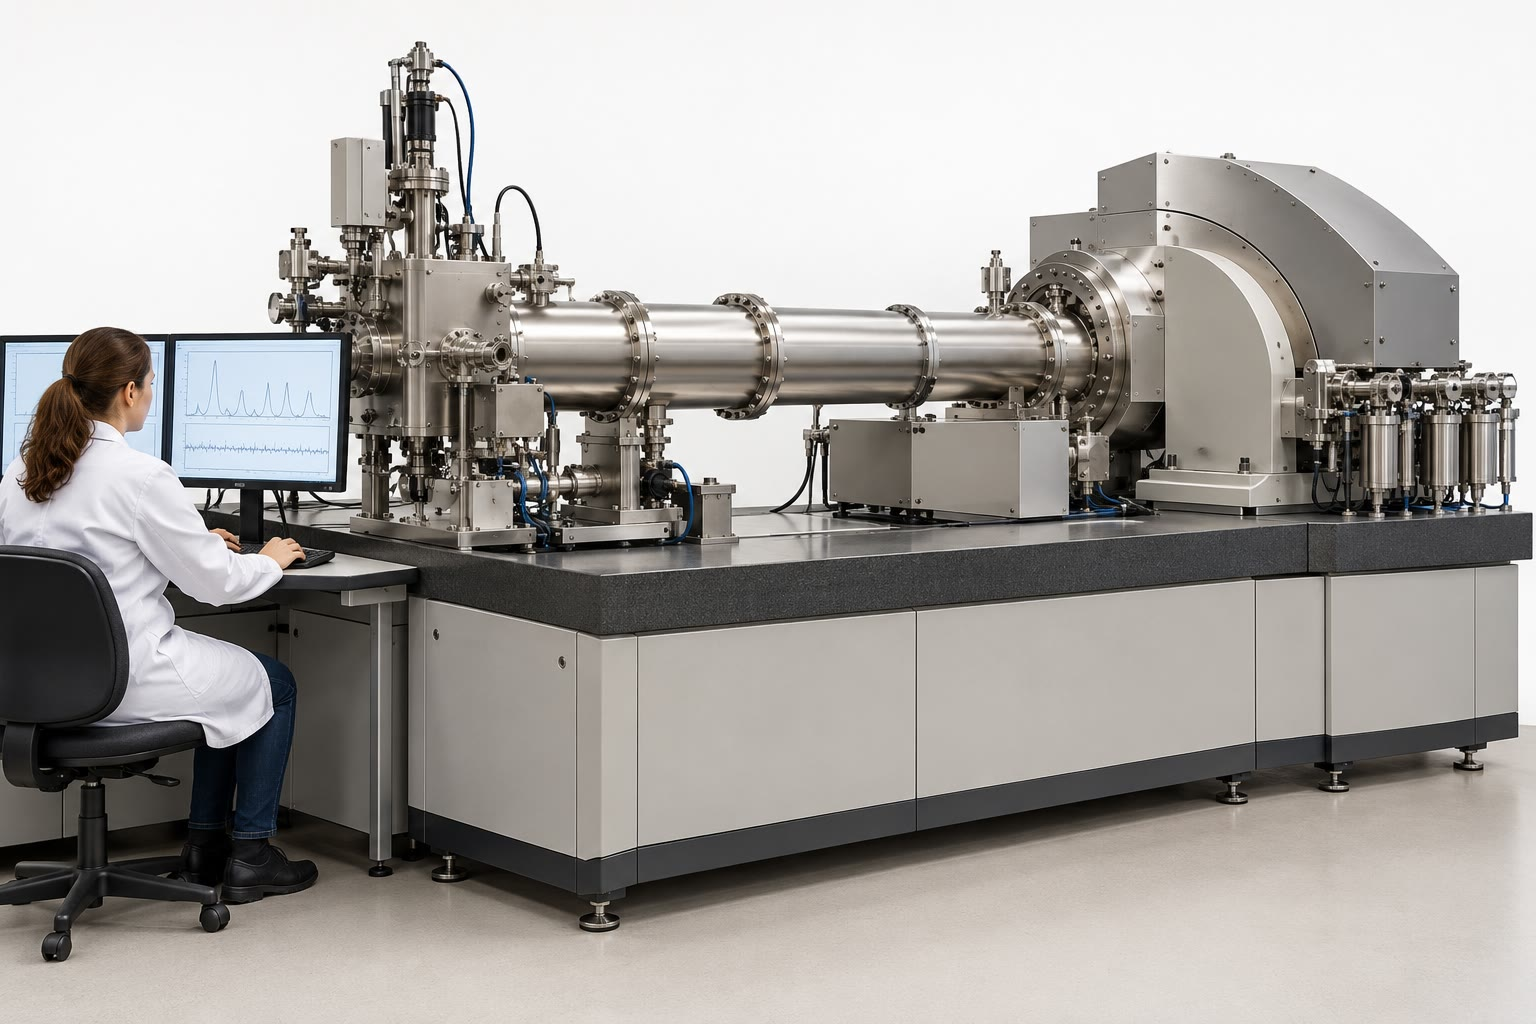
\includegraphics[width=\linewidth]{images/book4/ai/b2-isotope-lab.jpg}
\par\smallskip{\scriptsize 同位素实验室中的多接收器质谱仪
（AI 生成插图）。}
\end{minipage}
\end{inthelab}
% ledger: white:chur

\section{练习}

\begin{exercise}[$\star$]\label{exo:b2:isotope-geochemistry:1}
一块取自特里斯坦-达库尼亚群岛的玄武岩，其 $^{143}\mathrm{Nd}/^{144}\mathrm{Nd} = 0.51249$，另一块
取自芒阿伊岛，比值为 0.51285。求二者的 $\varepsilon_{\mathrm{Nd}}$ 以及平均
MORB（0.513074）的该值。哪些源区的 Sm/Nd 比值高于\omterm{def:b2:planet-formation-meteorites:chondrule}{球粒陨石}？
\end{exercise}

\begin{exercise}[$\star$]\label{exo:b2:isotope-geochemistry:2}
$^{18}\mathrm{O}/^{16}\mathrm{O}$ 的比值在 \omterm{def:b2:isotope-geochemistry:standards}{VSMOW} 中为 \num{2.0052e-3}，
在 \omterm{def:b2:isotope-geochemistry:standards}{VPDB} 中为 \num{2.0672e-3}。求 \omterm{def:b2:isotope-geochemistry:standards}{VPDB} 在 \omterm{def:b2:isotope-geochemistry:standards}{VSMOW} 标度上的 $\delta^{18}\mathrm{O}$ 值是多少？
一块方解石的 $\delta^{18}\mathrm{O} = -2.0$‰（相对 \omterm{def:b2:isotope-geochemistry:standards}{VPDB}），求其比值
及其在 \omterm{def:b2:isotope-geochemistry:standards}{VSMOW} 标度上的 $\delta^{18}\mathrm{O}$。
\end{exercise}

\begin{exercise}[$\star$]\label{exo:b2:isotope-geochemistry:3}
求 CHUR 在 \qty{1.0}{Ga} 前和
\qty{4.567}{Ga} 前的 $^{143}\mathrm{Nd}/^{144}\mathrm{Nd}$（$\lambda_{147} = \qty{6.524e-12}{\per\year}$，
$^{147}\mathrm{Sm}/^{144}\mathrm{Nd} = 0.1966$，今天为 0.512638）。
\end{exercise}

\begin{exercise}[$\star$]\label{exo:b2:isotope-geochemistry:4}
某山地气象站的雪样品 $\delta^{18}\mathrm{O} = -18.0$‰。
\omterm{prop:b2:isotope-geochemistry:mwl}{大气降水线}预测其 $\delta\mathrm{D}$ 为多少？一湖水的
$\delta^{18}\mathrm{O} = -4.0$，$\delta\mathrm{D} = -42$‰，求其氘
过量 $d = \delta\mathrm{D} - 8\delta^{18}\mathrm{O}$，并说明它位于该线之上还是
之下。
\end{exercise}

\begin{exercise}[$\star\star$]\label{exo:b2:isotope-geochemistry:5}
计算线性生长命题的 $Q$。一花岗岩中 Sm 为 \qty{6.0}{ppm}，
Nd 为 \qty{30}{ppm}（CI：0.145 和 \qty{0.457}{ppm}）。求其
$f_{\mathrm{Sm/Nd}}$，以及其 $\varepsilon_{\mathrm{Nd}}$ 在
\qty{500}{Ma} 内的变化量。
\end{exercise}

\begin{exercise}[$\star\star$]\label{exo:b2:isotope-geochemistry:6}
某地壳于 \qty{2.7}{Ga} 前从
$\varepsilon_{\mathrm{Nd}} = +3.5$ 的地幔中分离出来，其 $f_{\mathrm{Sm/Nd}} = -0.45$。用线性生长命题估计其
今天的 $\varepsilon_{\mathrm{Nd}}$。精确计算得 $-27.3$，
近似值与之相差多少，
为何偏高或偏低？
\end{exercise}

\begin{exercise}[$\star\star$]\label{exo:b2:isotope-geochemistry:7}
一玄武质岩浆（Sr 为 \qty{130}{ppm}，$^{87}\mathrm{Sr}/^{86}\mathrm{Sr} = 0.7030$）
同化了一花岗岩（Sr 为 \qty{320}{ppm}，0.7200）。计算含
5\%、10\% 和 20\% 花岗岩的混合物的 $^{87}\mathrm{Sr}/^{86}\mathrm{Sr}$。
证明 $^{87}\mathrm{Sr}/^{86}\mathrm{Sr}$ 相对于 $1/\mathrm{Sr}$ 为一条直线，
并求其斜率和截距。
\end{exercise}

\begin{exercise}[$\star\star$]\label{exo:b2:isotope-geochemistry:8}
以液-汽分馏系数 1.0098（$^{18}$O）和 1.084（D）
在 \qty{20}{\degreeCelsius} 下，计算与海水（0, 0）平衡的水汽的
$\delta^{18}\mathrm{O}$ 和 $\delta\mathrm{D}$，以及从水到水汽连线的斜率
$\delta\mathrm{D}/\delta^{18}\mathrm{O}$。在 \qty{0}{\degreeCelsius}（1.0117 和 1.111）下重复计算，
并与\omterm{prop:b2:isotope-geochemistry:mwl}{大气降水线}作比较。
\end{exercise}

\begin{exercise}[$\star\star$]\label{exo:b2:isotope-geochemistry:9}
大陆地壳占硅酸盐地球质量的 0.51\%，平均含
\qty{27}{ppm} 的 Nd，硅酸盐地球则为 \qty{1.25}{ppm}。取地壳的
$\varepsilon_{\mathrm{Nd}}$ 为 $-15$，硅酸盐地球的为 0。地壳持有钕的
份额是多少？若其余地幔均匀，
其 $\varepsilon_{\mathrm{Nd}}$ 应为多少？若其余地幔为\omterm{def:b2:planet-formation-meteorites:chondrule}{球粒陨石}型，
一个 $+8.5$ 的亏损储库须持有多少份额的钕？
\end{exercise}

\begin{exercise}[$\star\star\star$]\label{exo:b2:isotope-geochemistry:10}
证明：在线性生长命题中，被略去的项的相对大小约为
$\lambda t/2$。以地球年龄计，该值有多大，
并由此在 $\varepsilon_{\mathrm{Nd}}$ 上造成多大误差（$f = -0.45$，
历时 \qty{2.7}{Ga}）？
\end{exercise}

\begin{exercise}[$\star\star\star$]\label{exo:b2:isotope-geochemistry:11}
两端元的 Sr/Nd 比值分别为 13.3（A）和 5.0（B）。利用\omterm{prop:b2:isotope-geochemistry:mixing}{混合双曲线}的证明，
求混合物中来自 A 的锶的份额 $s'$，该混合物中 A
提供钕的份额 $s = 0.5$。对于哪个 $s$ 值，两者的份额
相差最大？
\end{exercise}

\begin{exercise}[$\star\star\star$]\label{exo:b2:isotope-geochemistry:12}
箱式模型给出，自地球于 \qty{4.5}{Ga} 前形成以来生成的大陆地壳，
其量为现今体积（\qty{7.2e9}{km^3}）的 2.3 至 2.6 倍，被破坏的量为 1.3 至 1.6 倍。
求生成与破坏的平均速率（单位
\unit{km^3}/年），并与俯冲带现今的速率比较，
即每年新增 \qty{2.7}{km^3}，每年移除 \qty{3.2}{km^3}。
\end{exercise}

\section{问题：三座岛屿，三种地幔}

\begin{problem}[{周末问题——将三座岛屿的熔岩置于地幔阵列上，
分离出混合物中的第三端元，并测定
再循环沉积物的年龄}]
\label{pb:b2:isotope-geochemistry:1}
假想大洋中的三座火山岛科拉、韦尔和阿沙喷发出玄武岩，
其同位素比值如下。地球化学家用两种成分模拟其源区：
一种类似 MORB 源区的\omterm{def:b2:isotope-geochemistry:reservoirs}{亏损地幔}（Sr 为 \qty{10}{ppm}，Nd
为 \qty{0.75}{ppm}，$^{87}\mathrm{Sr}/^{86}\mathrm{Sr} = 0.70282$，
$^{143}\mathrm{Nd}/^{144}\mathrm{Nd} = 0.51307$）和一种经俯冲返回地幔的
古老沉积物（Sr 为 \qty{200}{ppm}，Nd 为 \qty{40}{ppm}，$0.72000$，$0.51141$；
$^{147}\mathrm{Sm}/^{144}\mathrm{Nd} = 0.110$，$^{87}\mathrm{Rb}/^{86}\mathrm{Sr} = 0.50$）。
科拉：$0.70410$，$0.51278$；韦尔：$0.70618$，$0.51242$；阿沙：$0.70290$，$0.51288$
（$^{87}\mathrm{Sr}/^{86}\mathrm{Sr}$，$^{143}\mathrm{Nd}/^{144}\mathrm{Nd}$）。今天的 CHUR：
$^{143}\mathrm{Nd}/^{144}\mathrm{Nd} = 0.512638$，$^{147}\mathrm{Sm}/^{144}\mathrm{Nd} =
0.1966$；$\lambda_{147} = \qty{6.524e-12}{\per\year}$，$\lambda_{87} =
\qty{1.3972e-11}{\per\year}$。

\medskip\noindent\textbf{第一部分——岛屿定位。}
\begin{enumerate}
\item 求两种成分的 $\varepsilon_{\mathrm{Nd}}$。
\item 求三座岛屿的 $\varepsilon_{\mathrm{Nd}}$。
\item 将五种组成点绘于 Sr--$\varepsilon_{\mathrm{Nd}}$ 图上。哪些
岛屿位于 CHUR 的富集一侧？
\item 阿沙的锶比值与\omterm{def:b2:isotope-geochemistry:reservoirs}{亏损地幔}几乎相同，但
$\varepsilon_{\mathrm{Nd}}$ 低得多。它相对地幔阵列落在何处，
它与本章哪一岛群相似？
\item 为什么可以把熔岩的同位素比值当作其源区的比值，
尽管熔岩的 Sm/Nd 和 Rb/Sr 与其源区相差很大？
\item 科拉岛的一块熔岩，$^{147}\mathrm{Sm}/^{144}\mathrm{Nd} = 0.12$，年龄为 \qty{1}{Ma}。
自喷发以来，其 $^{143}\mathrm{Nd}/^{144}\mathrm{Nd}$ 增长了多少，
以 ε 单位计？这一点重要吗？
\end{enumerate}

\noindent\textbf{第二部分——两种组分的混合。}
\begin{enumerate}[resume]
\item 写出混合物的 Nd 浓度和 $^{143}\mathrm{Nd}/^{144}\mathrm{Nd}$，
其中沉积物质量分数为 $f$。
\item 计算混合物的 $\varepsilon_{\mathrm{Nd}}$，
沉积物质量分数分别为 $f = 0.5$、1、2 和 5\%。
\item 计算相同混合物的 $^{87}\mathrm{Sr}/^{86}\mathrm{Sr}$。
\item 证明混合物的 $^{87}\mathrm{Sr}/^{86}\mathrm{Sr}$
随 $1/\mathrm{Sr}$ 呈直线关系，并给出其斜率。
\item 计算 $K = (\mathrm{Sr}/\mathrm{Nd})_{\text{地幔}}/(\mathrm{Sr}/\mathrm{Nd})_{\text{沉积物}}$。
随着 $f$ 增大，Sr 与 Nd 两个比值中哪一个更快地向沉积物方向移动？
\item 沉积物中 Nd 和 Sr 的含量分别是地幔的多少倍？
利用这些数字解释为什么 1\% 的沉积物会使
$\varepsilon_{\mathrm{Nd}}$ 改变约 11 个单位。
\item 沉积物质量分数为 $f = 1$\% 的混合物中，
有多大比例的钕来自沉积物？
\end{enumerate}

\noindent\textbf{第三部分——需要多少沉积物？}
\begin{enumerate}[resume]
\item 对 Nd 混合方程求解 $f$，已知混合物的比值 $R$。
\item 利用 Kora 的钕含量计算其 $f$。
\item 利用 Kora 的锶含量计算其 $f$。两者是否一致？
\item 分别利用 Vel 的钕含量和锶含量计算其 $f$。
\item 利用 Asha 的钕含量计算其 $f$，并由该 $f$
预测锶同位素比值，并与实测值比较。
关于 Asha 的源区，你能得出什么结论？
\item 从本章中给出 Asha 的第三个组分，
并说明它必须具有的母体与子体比值。
\end{enumerate}

\noindent\textbf{第四部分——沉积物的年龄。}
\begin{enumerate}[resume]
\item 沉积物于 \qty{2.0}{Ga} 前俯冲，此后一直处于封闭状态。
计算沉积物在该时刻的 $^{143}\mathrm{Nd}/^{144}\mathrm{Nd}$、CHUR 的同一比值以及
该时刻的 $\varepsilon_{\mathrm{Nd}}$。
\item 用线性增长命题重做该计算。
\item 计算 \qty{2.0}{Ga} 前沉积物的 $^{87}\mathrm{Sr}/^{86}\mathrm{Sr}$。
\item \qty{2.0}{Ga} 前，$\varepsilon_{\mathrm{Nd}}$ 图中的地壳
具有 $\varepsilon_{\mathrm{Nd}} \approx -4.7$。俯冲时沉积物的数值
是否与其源自这种较年轻大陆地壳的侵蚀作用相符？
\item 陈述最富集岛屿源区中再循环沉积物的
质量分数，这是本题的关键数值。
\end{enumerate}
\end{problem}
% ledger: white:chur, villa20:sm147, villa22:rb87, gale13:isotopes
